\newpage
\section{Execution and Results} \label{sec:results}
    \subsection{Optimization of Settings}
    Before we started with the actual measurements, we optimized the settings.
    First parameter $\Delta m$, resolution \texttt{res} and acceleration voltage $U$ had to be chosen optimally. Secondly, the two detector types Faraday and SEM were compared. Finally residual gas spectrum of the vacuum chamber was recorded for different settings. Since we assume that the residual gas consists primarily of air, we excluded atoms heavier than 50~amu and limited our scans to the range of 1 amu/e to 50 amu/e. For the step sizes we chose 0.2 amu/e and carried out seven measurement runs. If nothing else is written, 70 V was selected as $U$.
    
    $\Delta m$ setting affects the offset of the work line. To optimize $\Delta m$ we set \texttt{res} = 0\% and performed measurements for $\Delta m = -10\%, -5\%, 0\%, 5\%, 10\%, 15\%, 20\%, 35\%$.  The curves for $\Delta m = -10\%, 5\%, 20\%, 35\%$ are shown in the figures \ref{fig:delta_m_variation} for the peak with the lowest and the largest measured mass-to-charge ratio.
    
    \begin{figure}[h!]
        \centering
        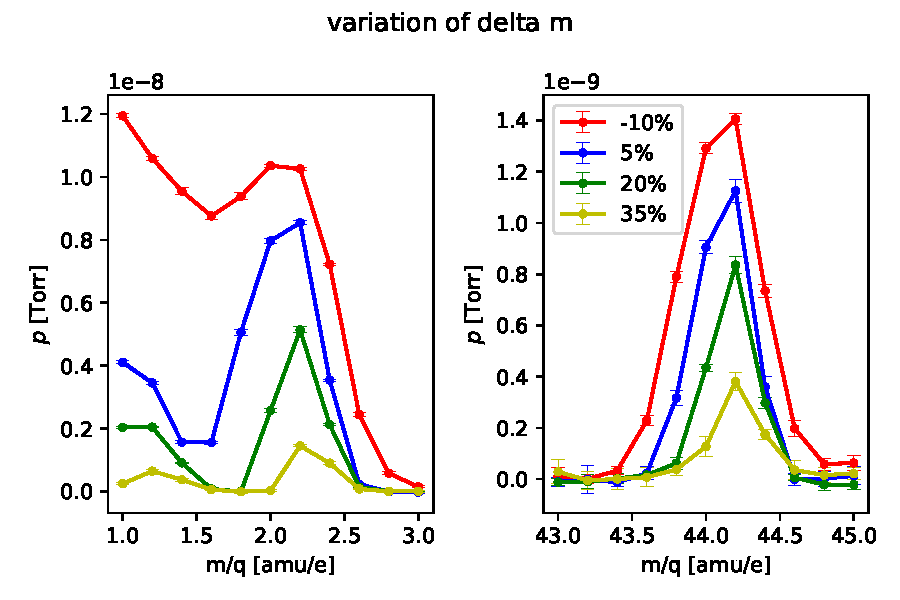
\includegraphics[width=1 \textwidth]{Report/DataResultsPlots/delta m_variation_h2_and_co2.pdf}
        \caption{$\Delta$m variation}
        \label{fig:delta_m_variation}
    \end{figure}
    
    When looking at these measurements we notice that the larger $\Delta m$ gets, the less pressure is measured. So the sensitivity decreases strongly with increasing $\Delta m$. Additionally we can see
    that the smaller $\Delta m$ is chosen, the wider the curves become. In order to avoid an overlapping of the individual curves in case of neighboring mass peaks, $\Delta m$ must not be too large. We chose $\Delta m= 20\%$ as the optimal mixture of sensitivity and curve width. The smaller the atomic mass-to-charge ratio, the stronger the sensitivity increases with decreasing $\Delta m$. This is especially visible in the range of $m/q$ = 1 amu/e, where the peak with decreasing $\Delta m$ becomes larger than the peak in the range of $m/q$ = 2 amu/e. This is in accordance with the descriptions of the parameter $\Delta m$ in the manual \cite{manual}. 
    
    To optimize \texttt{res}, which affects the slope of the work line, we chose $\Delta m = 20\%$ and varied \texttt{res} = -5\%, 5\%, 10\%. The results at the relevant ranges are shown in figure \ref{fig:resolution_variation}.
    
    \begin{figure}[h!]
        \centering
        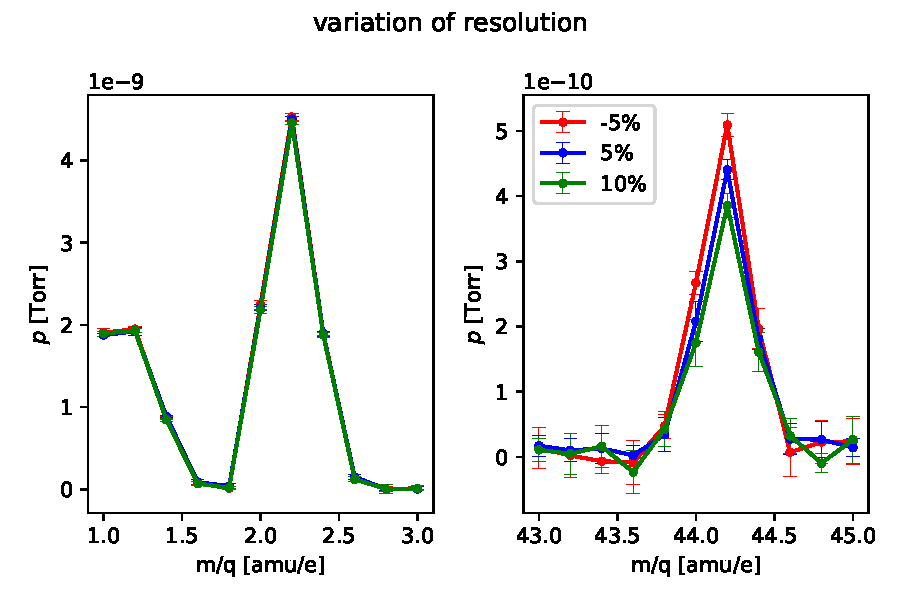
\includegraphics[width=1 \textwidth]{Report/DataResultsPlots/resolution_variation_h2_and_co2.pdf}
        \caption{resolution variation}
        \label{fig:resolution_variation}
    \end{figure}
    
    We find that \texttt{res} has hardly any influence on the sensitivity close to $m/q$ = 0 amu/e, but a clearly discernible influence in the range of $m/q$ = 44 amu/e. This fact was also described in the manual. Since \texttt{res} does not have a strong influence even in the larger range, we decided to set \texttt{res} in the later measurements neutral to 0\%. 
    
    To select the optimum $U$, $\Delta m = 20 \%$, \texttt{res} = 5\% was kept constant and the voltages of 50~V, 70~V and 90~V were tested. For most of the peaks the sensitivity was higher the lower the $U$ was (see \ref{fig:voltage_variation} on the right). This may have to do with the fact that at low voltage less double ionization occurs. Therefore we decided to use an $U$ of 50~V.  
    
    \begin{figure}[h!]
        \centering
        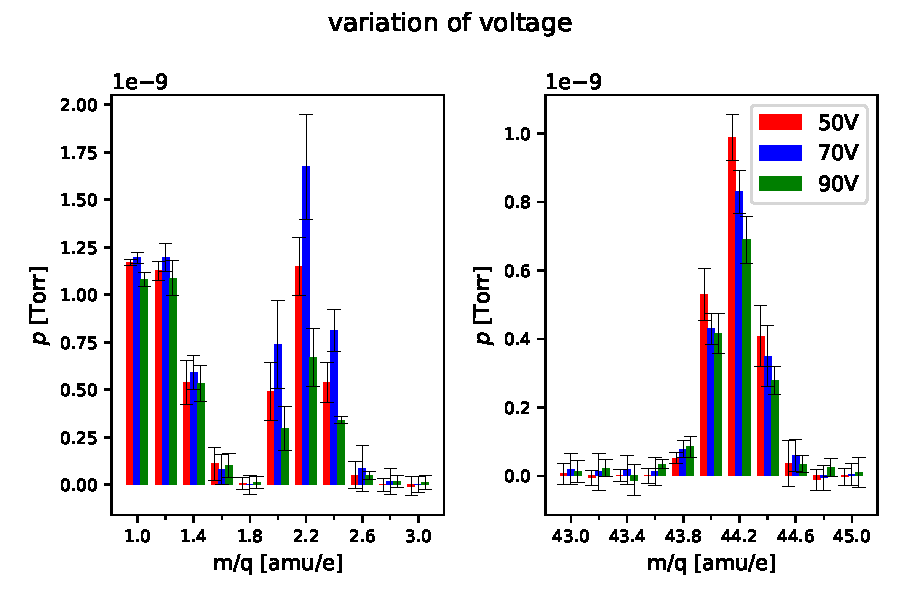
\includegraphics[width=1 \textwidth]{Report/DataResultsPlots/voltage_variation_h2_and_co2.pdf}
        \caption{voltage variation}
        \label{fig:voltage_variation}
    \end{figure}
    
    Finally we now come to compare the two detectors. For this purpose, both detectors were measured with \texttt{res} = 5\%, $\Delta m = 20\%$ and $U$ = 70~V. As we can see from the figure \ref{fig:detector_variation}, the sensitivity of the Faraday detector is significantly higher than that of the SEM. Therefore we decided to use the Faraday detector for our measurements. 
    \begin{figure}[h!]
        \centering
        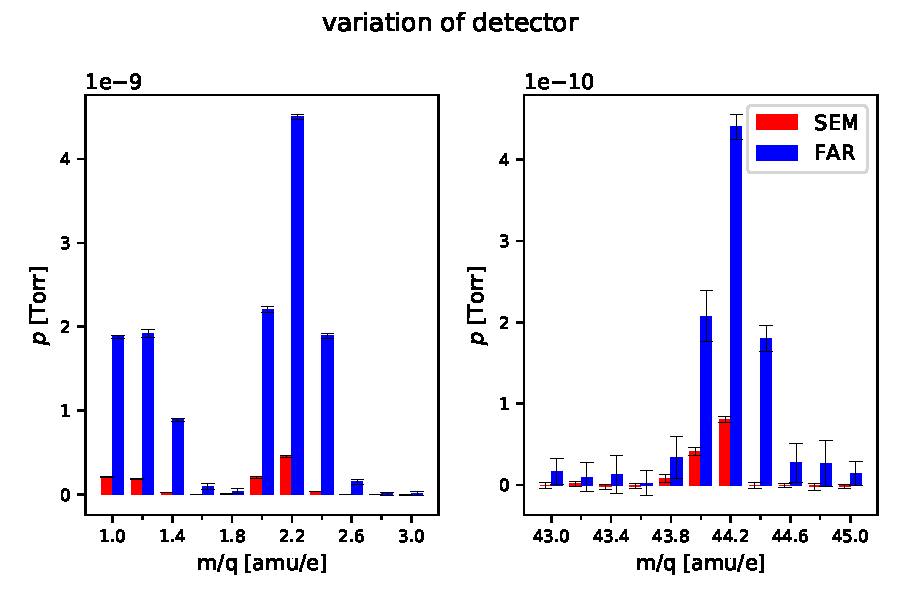
\includegraphics[width=1 \textwidth]{Report/DataResultsPlots/detector_variation_h2_and_co2.pdf}
        \caption{detector variation}
        \label{fig:detector_variation}
    \end{figure}
    
    
    In summary, the parameters are optimal if $\Delta m = 20\%$, \texttt{res} = 0\%, $U$ = 50~V and the Faraday detector is selected. 
    
    \newpage
    \subsection{Residual gas Identification}
    
    After the optimal settings were found, we performed a residual gas spectrum measurement from 1 amu/e to 140 amu/e. We refined the step size to 0.1 amu/e to have more measurement points for the {\scshape Gaussian} fits. Figure \ref{fig:residual_gas} shows the measured partial pressures and the detected gas components. Table \ref{table:residual gas} shows the abundance of the gases.
    
   

    \begin{figure}[h!]
        \centering
        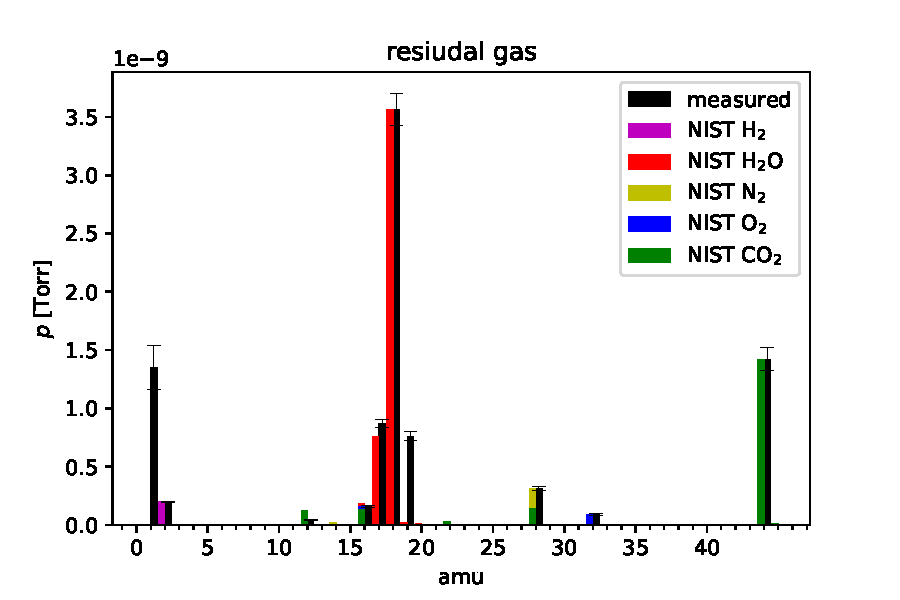
\includegraphics[width=0.6\textwidth]{Report/DataResultsPlots/resiudal gas.pdf}
        \caption{residual gas measurement compared to first kind of \texttt{NIST} approximation}
        \label{fig:residual_gas}
    \end{figure}
    
    \begin{table}[h!]
      \begin{center}
      \DTLsetseparator{,}
        \DTLloaddb[keys={substance,fraction,err}]{komp_residual}{komp_residual.csv}
        \begin{tabular}{l|c}
            \toprule substance & abundance [\%] 
            \DTLforeach{komp_residual}{\mat=substance,\a=fraction,\aerr=err}
            {\DTLiffirstrow{\\ \midrule}{\\}
            \mat & \pgfmathprintnumber[textnumber]\a~$\pm$~\pgfmathprintnumber[textnumber]\aerr}
            \\\bottomrule
        \end{tabular}
        \caption{Abundance of residual gas components, calculated using second kind of \text{NIST} approximation.}
        \label{table:residual gas}
      \end{center}
    \end{table}
    
     We detected CO$_2$, H$_2$0, N$_2$, O$_2$ and H$_2$. The large proportion of H$_2$O is striking. This gas has the property of condensing easily on the walls of the vacuum chamber and is therefore difficult to remove.
     
     N$_2$ and O$_2$ are both components of the air and get into the vacuum chamber again and again through leaks. As we can see in table \ref{table:residual gas}, their proportion is very close to each other although the ratio of these two substances in the air is 1/5. This may be due to their different masses, N$_2$ has a mass of 28 amu and O$_2$ has a mass of 32 amu. It is conceivable that smaller masses can be sucked out of the chamber better than heavier masses.
     
    The high partial pressure at 1 amu/e is also striking. This exceeds by far the value expected from the \texttt{NIST} approximation. This is due to an over-sensitivity of the mass spectrometer at 1 amu/e. As we noted in Figure \ref{fig:delta_m_variation}, $\Delta m$ has a strong influence on the sensitivity of small mass-to-charge ratios. Thus, the large partial pressure at 1 amu/e is not primarily due to H$_2$. However, the ratios in table \ref{table:residual gas} are calculated with the second kind of \texttt{NIST} approximation, whereby the entire partial pressure at 1 amu/e is attributed to H$_2$. As a result, the H$_2$ fraction is overestimated in this table.
    
    \subsection{Noble Gas Analysis}
    
    In this section, gas samples of the noble gases xenon, argon and an unknown noble gas mixture were analysed.
    for this purpose, these three gases were provided in gas cylinders. The cylinders could be connected to the system as shown in figure \ref{fig:cartridge}. 
    The mass spectra were plotted and the gas components of the samples were identified.  In the case of the gas mix, in addition to identifying the gas components, their ratio was determined.
    
    \begin{figure}[h!]
        \centering
        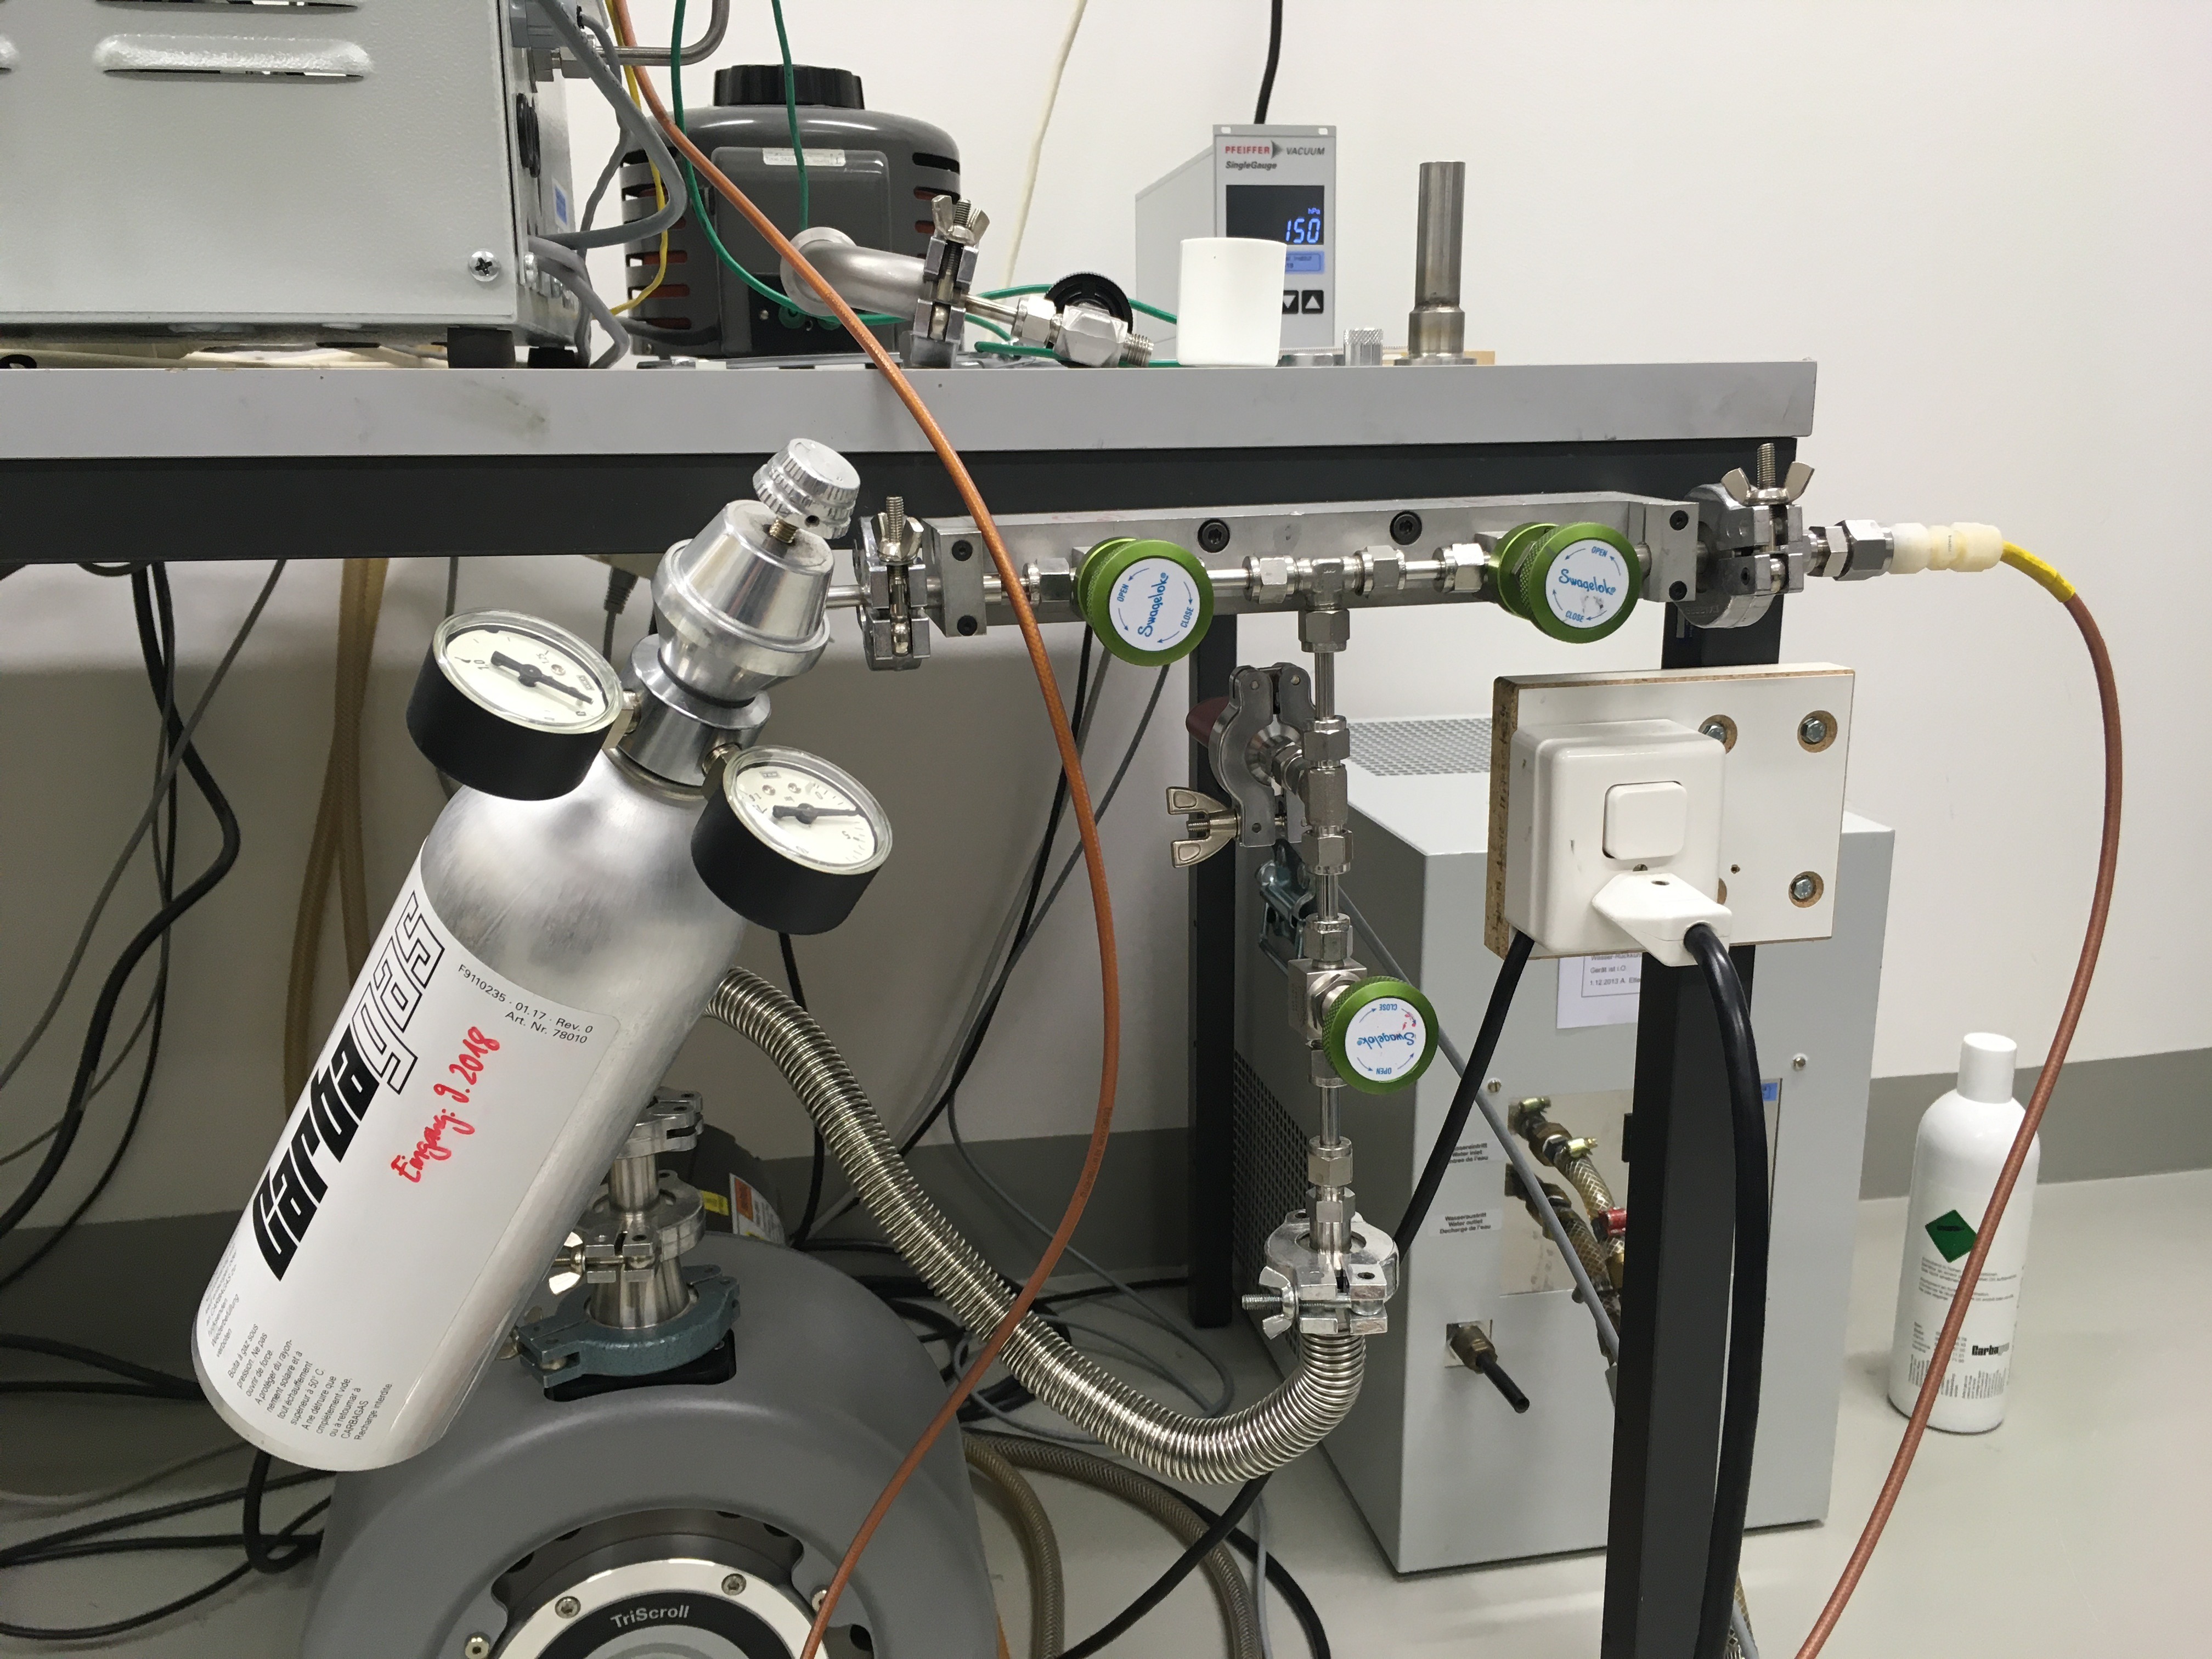
\includegraphics[width=0.6\textwidth]{Report/pictures/cartridge.JPG}
        \caption{The setup with an attached noble gas cylinder}
        \label{fig:cartridge}
    \end{figure}

    
    \begin{figure}[h!]
        \centering
        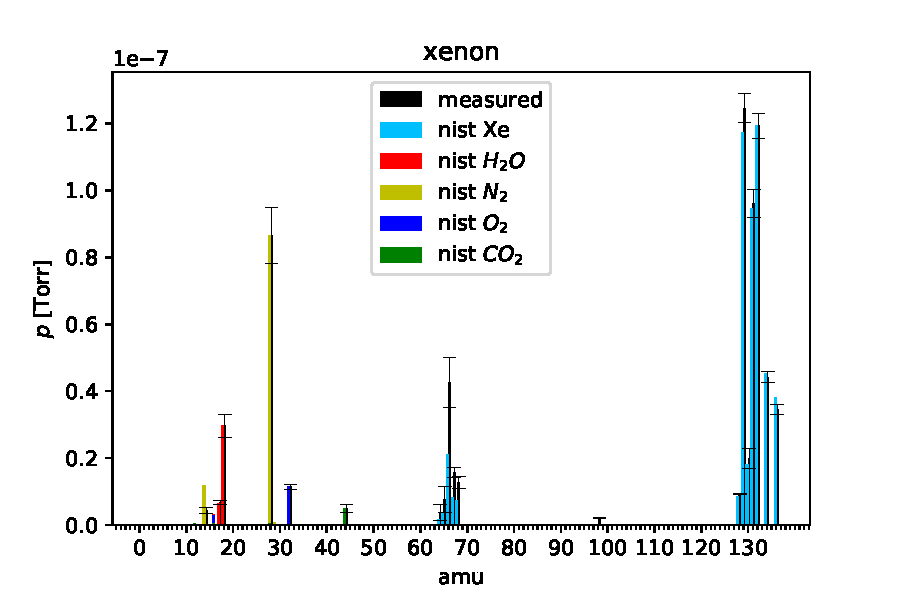
\includegraphics[width=0.6\textwidth]{Report/DataResultsPlots/Xenon.pdf}
        \caption{Xenon measurement compered to first kind of \texttt{NIST} approximation}
        \label{fig:xenon}
    \end{figure}
        As we can see in figure \ref{fig:xenon}
    all partial pressures of xenon, which should exist according to the \texttt{NIST} data, were confirmed by us. The partial pressures at half-integer mass-to-charge ratios were also calculated. However, for reasons of space, they are not entered in the plots. In the case of single ionisation for xenon, the \texttt{NIST} data approximations largely agree with the measured data. They are sometimes outside the error range, but only just. In addition, it must be taken into account that there is also an error in the scaling of the \texttt{NIST} ratios which is as large as that of $^{132}$Xe. The error of the \texttt{NIST} approximation is not entered to make the plots clearer. In the case of double ionised atoms, we measure larger values everywhere than would be expected. However, the number of double ionised atoms depends on the voltage $U$ and therefore does not necessarily correspond to the \text{NIST} ratios. Also noticeable are the N$_2$, O$_2$ and H$_2$O peaks that we find in the gas sample. The N$_2$ and O$_2$ molecules indicate that air also entered the pipes in addition to the gas sample.
    The peak at the 89 amu/e, we could not assign to any substance.
    
    \begin{figure}[h!]
        \centering
        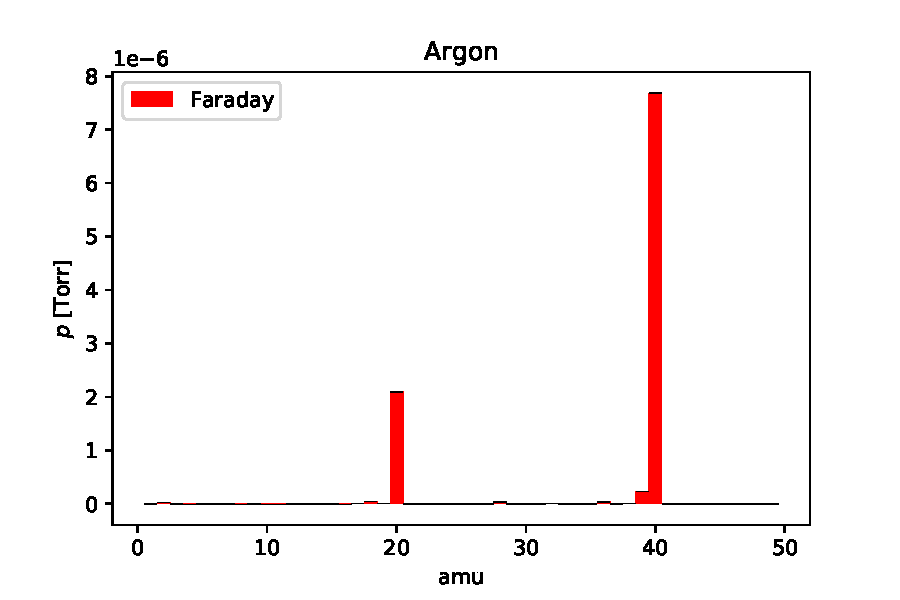
\includegraphics[width=0.6\textwidth]{Report/DataResultsPlots/Argon.pdf}
        \caption{Argon gas measurement compared to first kind of \texttt{NIST} approximation}
        \label{fig:argon}
    \end{figure}
   
    In the case of argon, we were also able to detect the most important peaks at 40 amu/e, 20 amu/e and 36 amu/e (figure \ref{fig:argon}). It is striking that the partial pressure at this measurement at 20 amu/e is very low, but looking at the plot of gas mix (figure \ref{fig:mix})  we see that the partial pressure at 20 amu/e agrees very well with the expected value. It is therefore not clear to us why we measure such a low partial pressure at this mass-to-charge ratio in the argon measurement. 
    
     
    \begin{figure}[h!]
        \centering
        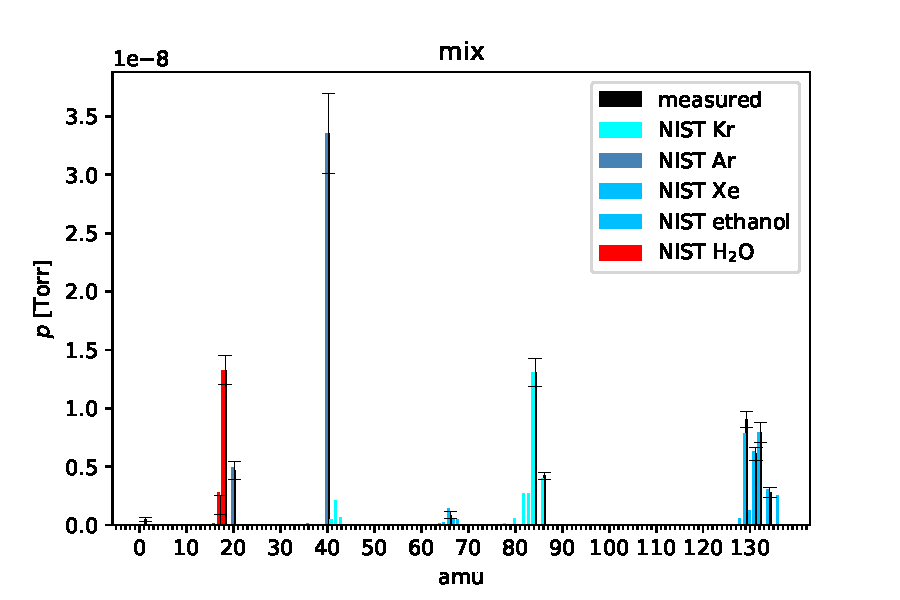
\includegraphics[width=0.6\textwidth]{Report/DataResultsPlots/mix.pdf}
        \caption{Measurement of an unknown gas mix}
        \label{fig:mix}
    \end{figure}
    
       For the gas mix, we find the components xenon, argon and krypton (figure \ref{fig:mix}). As already discussed, the partial pressures produced by argon agree very well with the expectations. For krypton and xenon, however, not all expected partial pressures are measured. The lack of these partial pressures could be related to the fact that in this measurement a much lower pressure in the vacuum chamber was chosen than in the xenon measurement, so that all partial pressures are much smaller (in the gas mix they are in the range of 10$^{-8}$ Torr and in xenon in the range of 10$^{-7}$ Torr). As a result, some peaks are so weak that they do not reach our threshold and are therefore not detected. This threshold is necessary to ensure that the peaks are clear enough to allow a {\scshape Gaussian} fit. Thus, the {\scshape Gaussian} fits provide a good method for determining well-defined partial pressures, but they have the disadvantage that weak partial pressures are not detected. In the table \ref{table:nobel_gas} the gas ratios of the gas mix determined by us can be seen. Apart from the already discussed problem that not all peaks were recognised, it is also possible that the different substance masses influence our result. It is quite conceivable that lighter atoms could escape more easily from the upright gas cylinder than the heavier ones. The alignment of the gas cylinder can be seen in figure \ref{fig:cartridge}. This would mean that our gas sample would not have exactly the same material ratio as the gas in the cylinder. In addition, the setting of the work line influences the sensitivity at the different mass-to-charge ratios. It is therefore very likely that the sensitivity is not exactly the same everywhere, this could strongly influence the calculated ratios. 
    
    \begin{table}[h!]
      \begin{center}
      \DTLsetseparator{,}
        \DTLloaddb[keys={substance,fraction,err}]{komp_mix}{komp_nobel_gas.csv}
        \begin{tabular}{l|c}
            \toprule substance & abundance [\%] 
            \DTLforeach{komp_mix}{\mat=substance,\a=fraction,\aerr=err}
            {\DTLiffirstrow{\\ \midrule}{\\}
            \mat & \pgfmathprintnumber[textnumber]\a~$\pm$~\pgfmathprintnumber[textnumber]\aerr}
            \\\bottomrule
        \end{tabular}
        \caption{Gas components in the gas mix and their proportions}
        \label{table:nobel_gas}
      \end{center}
    \end{table}
    

    \subsection{Isotope ratios in noble gases}
    In this part the measurements of the last subsection are used to determine the isotope ratio for the noble gases xenon, argon and krypton (see tables \ref{table:xenon_isotope}, \ref{table:argon_isotope} and \ref{table:krypton_isotope}). For each measured value, a literature value was also approached for comparison \cite{isotopes}.
    Since no separate gas sample was available for krypton, the isotope ratio for krypton was determined using the gas mix measurement. 
    
    To correctly estimate the partial pressure of an isotope, the partial pressure of both the single and the double ionised isotope must be taken into account. The mass-to-charge ratio of a double ionised isotope is half that of the single ionised isotope. If both partial pressures are added together, the total partial pressure of the isotope is obtained. The mass-to-charge ratio of a double-ionised isotope does not have to be an integer. Such peaks are also considered in the calculations, although they are not shown in the plots. 
    
    \begin{table}[h!]
     \begin{center}
      \DTLsetseparator{,}
        \DTLloaddb[keys={Isotop,fraction,err,lit}]{xenon_isotop}{isotop_xenon.csv}
        \begin{tabular}{l|c|c}
            \toprule isotope & abundance [\%] & literature  [\%]
            \DTLforeach{xenon_isotop}{\mat=Isotop,\a=fraction,\aerr=err, \b=lit}
            {\DTLiffirstrow{\\ \midrule}{\\}
             Xe \mat  & \pgfmathprintnumber[textnumber]\a~$\pm$~\pgfmathprintnumber[textnumber]\aerr & \b} 
            \\\bottomrule
        \end{tabular}
        \caption{Xenon isotopes}
        \label{table:xenon_isotope}
      \end{center}
    \end{table}
    
    As we can see in table \ref{table:xenon_isotope}, the literature values for xenon agree very well with the ratios we determined. The deviations from the literature values could possibly be due to the settings chosen in the mass spectrometer. These were selected so that the peaks are as clearly visible as possible, but they are not tested to ensure that they are equally sensitive at all mass-to-charge ratios.  
    
    \begin{table}[h!]
     \begin{center}
      \DTLsetseparator{,}
        \DTLloaddb[keys={Isotop,fraction,err,lit}]{argon_isotop}{isotop_argon.csv}
        \begin{tabular}{l|c|c}
            \toprule isotope & abundance [\%] & literature  [\%]
            \DTLforeach{argon_isotop}{\mat=Isotop,\a=fraction,\aerr=err, \b=lit}
            {\DTLiffirstrow{\\ \midrule}{\\}
            Ar \mat & \pgfmathprintnumber[textnumber]\a~$\pm$~\pgfmathprintnumber[textnumber]\aerr & \b}
            \\\bottomrule
        \end{tabular}
        \caption{Argon isotopes}
        \label{table:argon_isotope}
      \end{center}
    \end{table}
    
    In the case of argon isotopes in table \ref{table:argon_isotope}, the abundance deviate slightly from the literature values in case of $^{36}$Ar. Nevertheless, it is astonishing that we were able to measure this value even though its proportion is so small. Its deviation could be due, among other things, to the fact that very little partial pressure was measured at 20 amu/e in the argon measurement, as already discussed in the last subsection. If there was a higher measurement value, more $^{40}$Ar isotopes would have been detected and the ratio would shift. One isotope that we did not detect is $^{38}$Ar, but since it only accounts for 0.07\%, it is hardly detectable and its absence hardly influences our results.

    
    \begin{table}[h!]
     \begin{center}
      \DTLsetseparator{,}
        \DTLloaddb[keys={Isotop,fraction,err,lit}]{krypton_isotop}{isotop_krypton.csv}
        \begin{tabular}{l|c|c}
            \toprule isotope & abundance [\%] & literature  [\%]
            \DTLforeach{krypton_isotop}{\mat=Isotop,\a=fraction,\aerr=err, \b=lit}
            {\DTLiffirstrow{\\ \midrule}{\\}
             Kr \mat & \pgfmathprintnumber[textnumber]\a~$\pm$~\pgfmathprintnumber[textnumber]\aerr & \b}
            \\\bottomrule
        \end{tabular}
        \caption{Krypton isotopes}
        \label{table:krypton_isotope}
      \end{center}
    \end{table}
    
    When looking at the krypton isotopes in table \ref{table:krypton_isotope}, we notice strong deviations from the literature values. This is not surprising, however, since only two of the six possible isotopes were detected. We have already discussed the reasons for the lack of these partial pressures in the upper subsection.  It is worthwhile to check whether the ratio between $^{86}$Kr and $^{84}$Kr nevertheless agrees with the ratio in literature. We obtain for the ratio in theory $17.3/(17.3+57) = 23.28 \%$ which actually agrees with our measurements for $^{86}$Kr. This confirms our assumption that the detected peaks provide very good values, but that many too weak peaks could not be detected.
 


    \newpage

    \subsection{Inhaled Air}
    To compare the amount of carbon-dioxide and oxygen in exhaled air, one of us exhaled air into a balloon, attached it to the system and performed a measurement. Afterwards, one of us inhaled the air again and exhaled it again into the balloon. We repeated this procedure 5 times. The system was flushed with normal air in between each measurement. The peaks of carbon dioxide and oxygen were fitted using a {\scshape Gaussian} as described in section \ref{sec:fit}. The integrated data is normalised over the total data-set and is shown with uncertainties in figure \ref{fig:air}. 

    \begin{figure}[h]
            \centering
            \subfloat[absolute amounts]{\label{figure:depth_profile_13.72}
                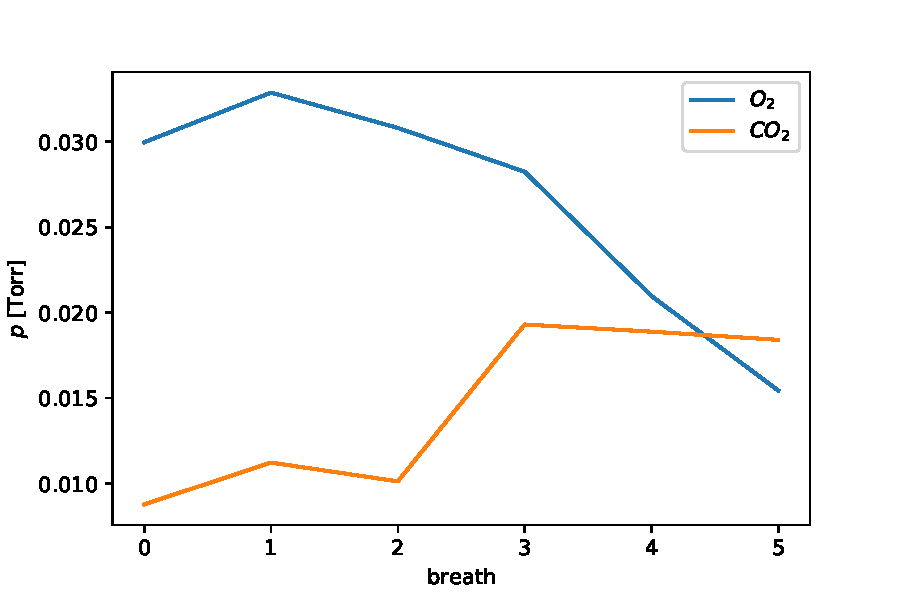
\includegraphics[width=0.47\textwidth]{Report/DataResultsPlots/air.pdf}}\quad
            \subfloat[relative amounts]{\label{figuer:zenith_13.72}
                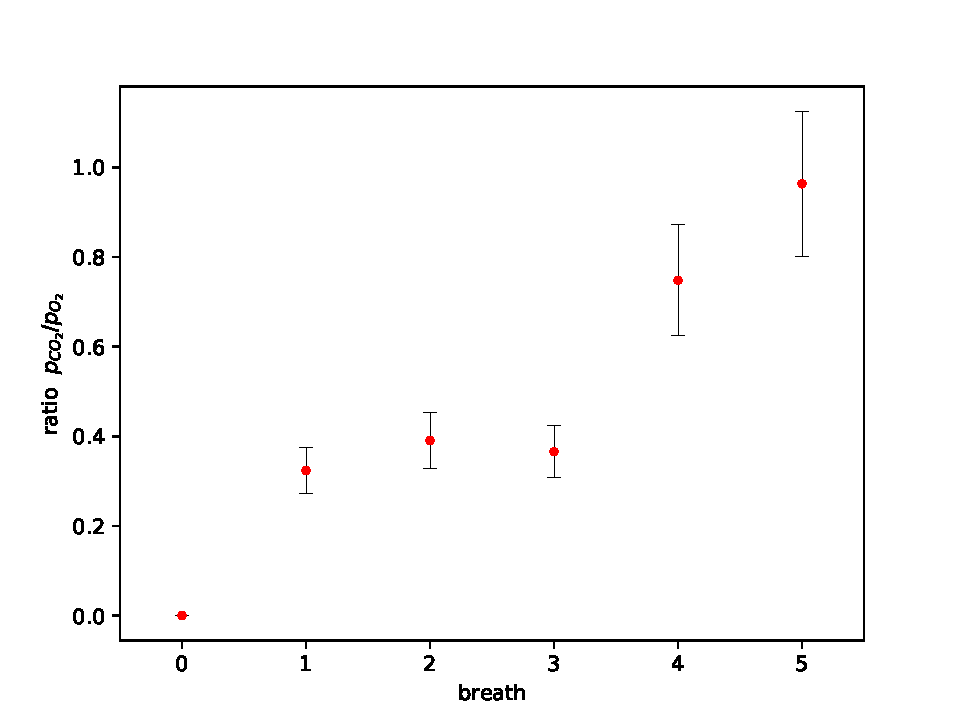
\includegraphics[width=0.47\textwidth]{Report/DataResultsPlots/air_relative.pdf}}\quad
            \caption{CO$_2$ and O$_2$ amount in Inhaled air.}
         \label{fig:air}
    \end{figure}
    
    
    To get an estimation of how much oxygen is actually converted into carbon dioxide we fit \eqref{eq:breath} to the oxygen set and \eqref{eq:breath2} to the carbon dioxide set.
    \begin{align}
        f_{\text{O}_2}(n) &= n_{\text{O}_2} \cdot p^n \label{eq:breath}\\
        f_{\text{CO}_2}(n) &= n_{\text{CO}_2} +  n_{\text{O}_2} - n_{\text{O}_2} \cdot p^n \label{eq:breath2}
    \end{align}
    We thus received the initial value of oxygen:
    $$ n_{\text{O}_2} = (14.17 \pm 1.97) \%$$
    And the initial value of carbon dioxide:
    $$ n_{\text{CO}_2} = (1.47 \pm 0.56) \%$$
    The two fits assume that the conversion ratio is 1:1. The high deviation of our datapoints from our fit is suspected to be due to the amount of nitrogen decreasing. The amount of Nitrogen is fluctuating between different measurements, and since nitrogen has a significant impact on the overall pressure, we see it directly in the normalised values for CO$_2$ and O$_2$ in the absolute amount plot. This correlation effect is also visible in  the relative plot where we plot the ratio of the amount of CO$_2$ and O$_2$. The factor $p$ we received from the fit is:
    $$p = (90.07 \pm 3.93) \;\text{per breath}$$
    This would suggest that around 9.93 $\pm$ 3.93 \% of the inhaled oxygen would be converted to carbon-dioxide during one breath.
    In reality, the oxygen amount decreases by about 4 to 5 \% per breath \cite{breath}.\\
    In figure \ref{fig:air}a we also notice that the error-bars on the oxygen measurements are significantly larger than the ones for the carbon-dioxide measurements. This is an indication that the system has not the same sensitivity for both components. Probably because the two components are not ionised equally well.
    In figure \ref{fig:air}b we see that the ratio of CO$_2$/O$_2$ increases and reaches 1. It follows a more or less linear pattern.
    
    
    \subsection{Measurement of Ethanol}
    
    In this experiment, we want to detect ethanol in different sources. First we tried with liquid ethanol and then with a sample of vodka. 
    A mass-spectrometer is only able to measure gaseous probes. Since Ethanol and vodka is liquid at room temperature, we had to attach a bent tube that is closed on the bottom after filling it with the liquid. After attaching it, we heated it with our hands to increase the amount of gaseous Ethanol entering the system. The setup is shown in figure \ref{fig:ethanol}.
    \begin{figure}[h!]
    \centering
    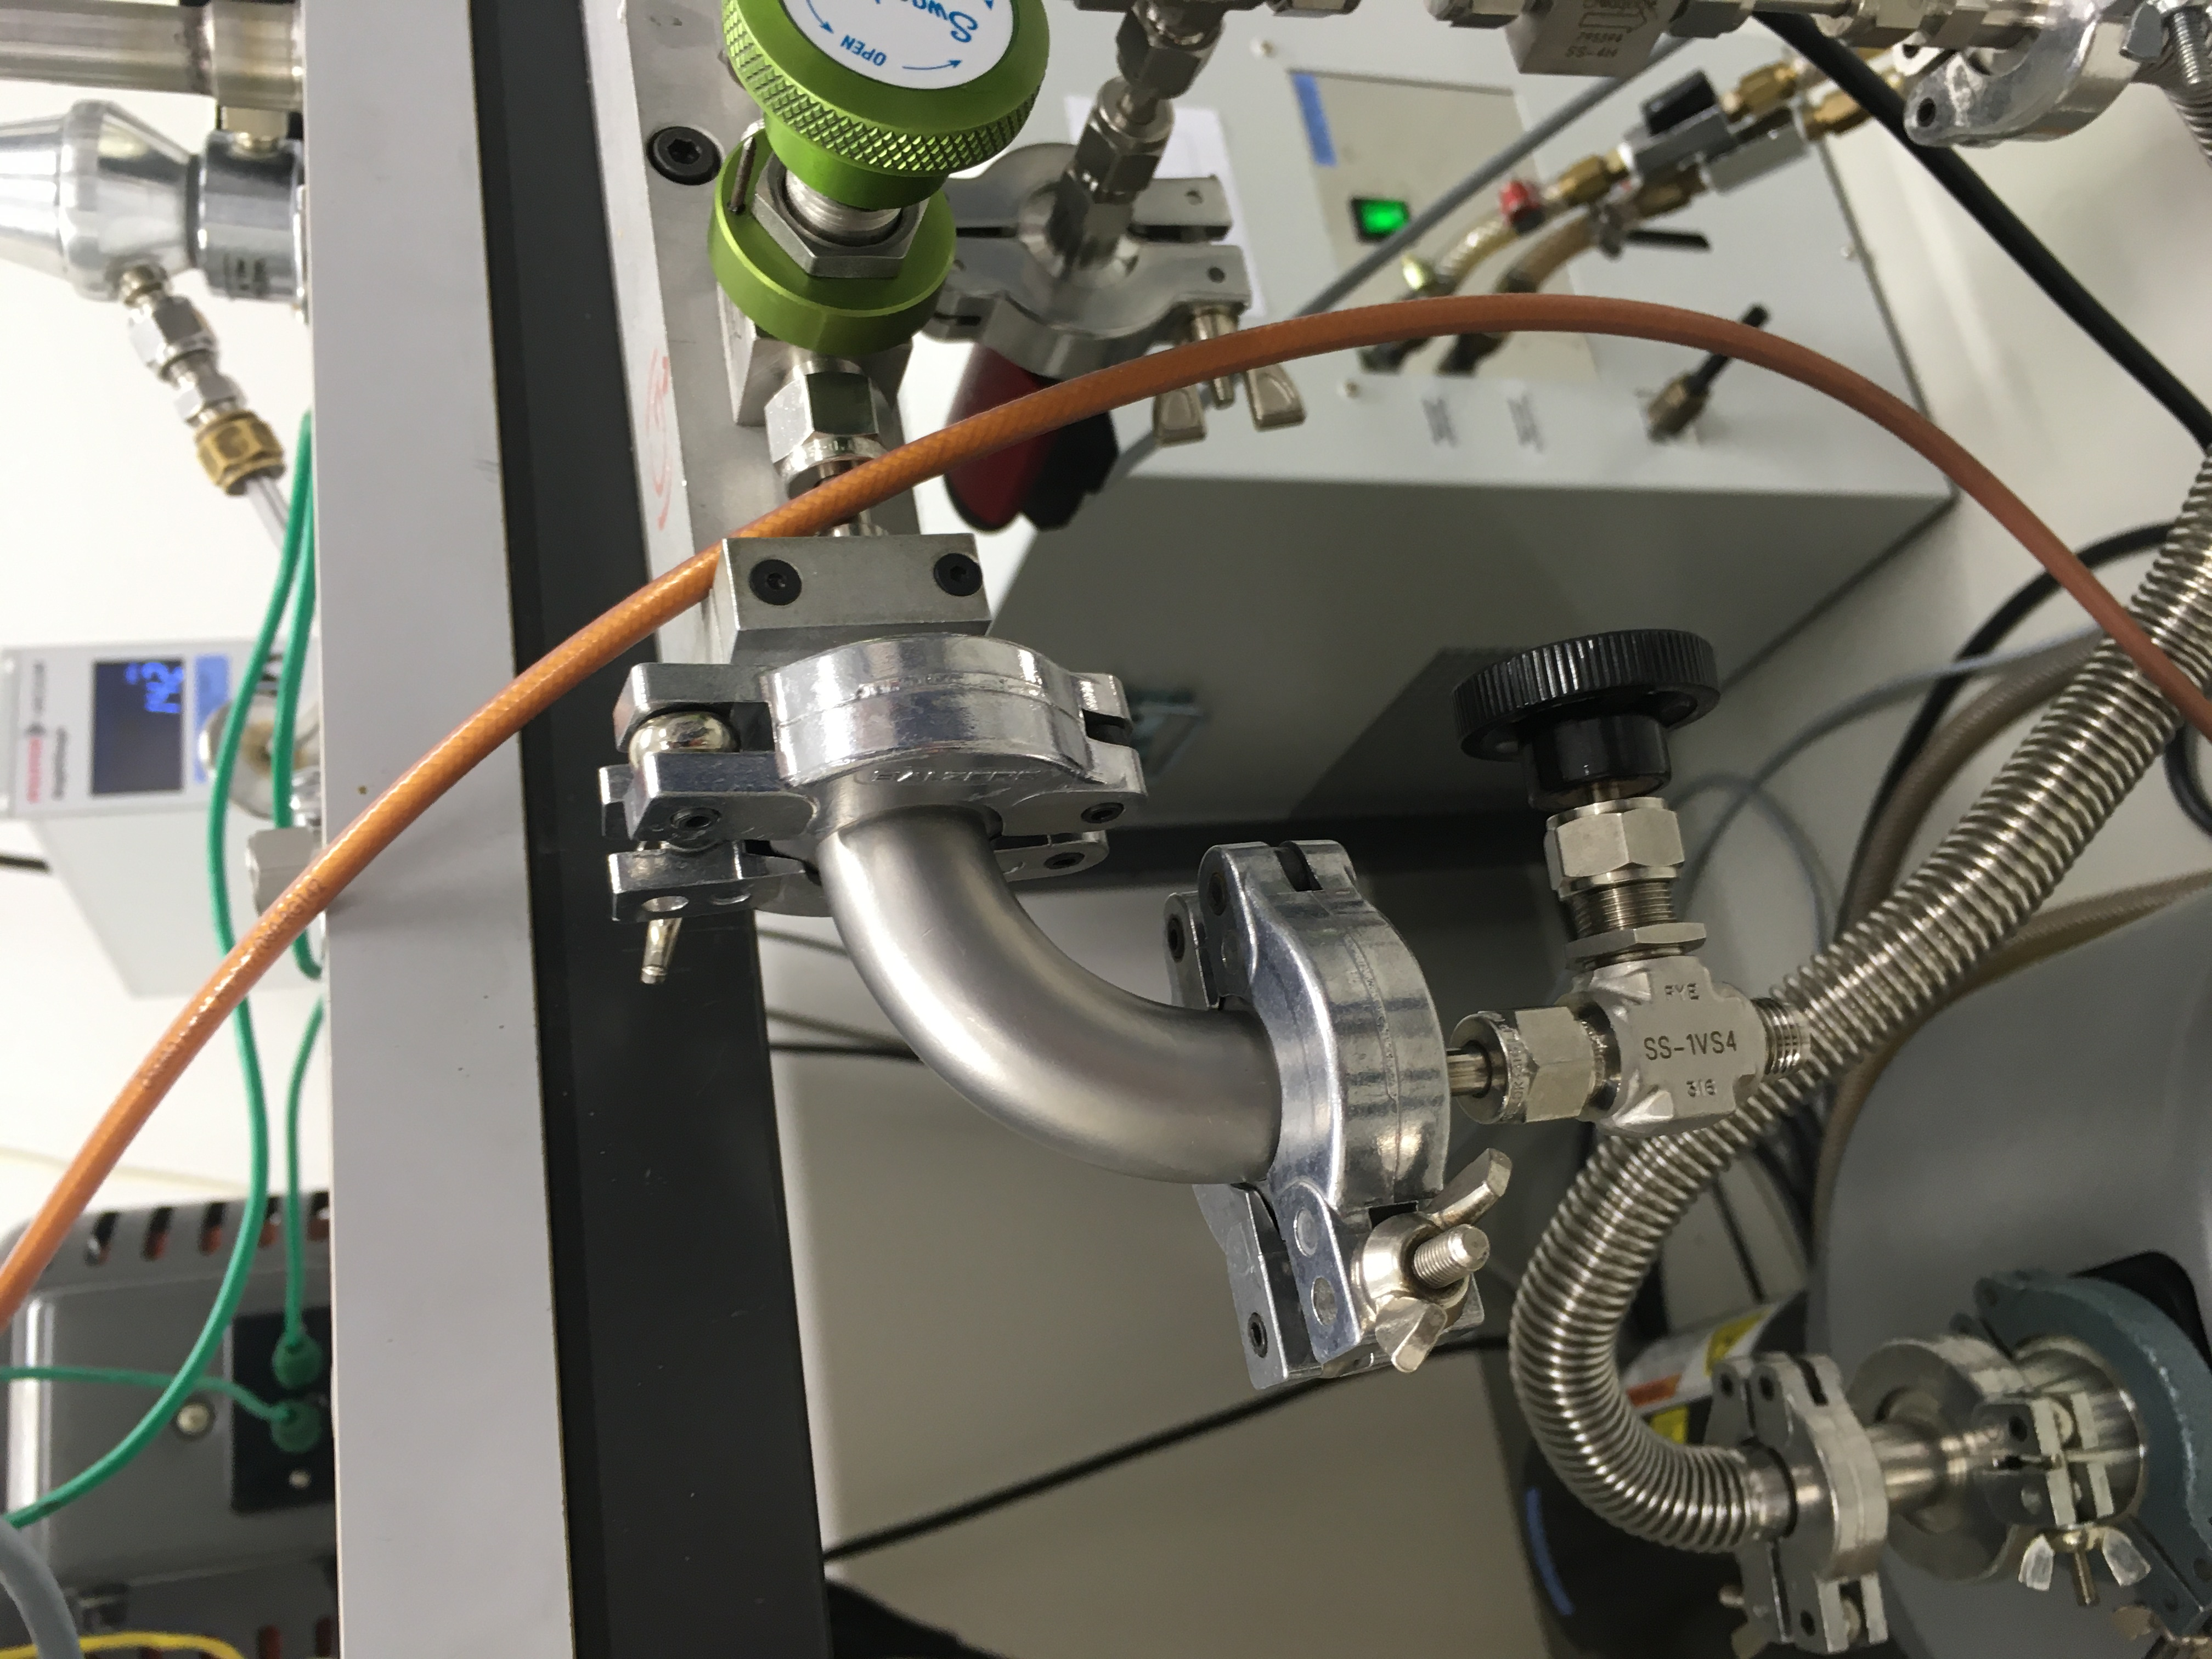
\includegraphics[angle=-90, origin=c,width=0.25\textwidth]{Report/pictures/liquids.JPG}
    \caption{The setup to attach a liquid sample to the system. The gaseous phase will be pumped to the mass spectrometer while the liquid phase will stay inside the container.}
    \label{fig:ethanol}
    \end{figure}
    Finally, a few sips of vodka were drunk and then the breath was blown into a balloon and connected to the mass spectrometer. We wanted to find out whether it is possible to detect alcohol in breath with this mass spectrometer. For the measurements of vodka and the alcohol breath, we chose measurement distances of 0.2 amu/e. The reason for this is that we first carried out all measurements with the large intervals and then repeated them with 0.1 amu. However, since we found that we did not detect any signs of ethanol peaks with vodka, the measurement was not repeated. Nevertheless, we would like to show the results of these measurements.
    
    The output of the ethanol measurement can be seen in figure \ref{fig:ethanol2}. As we can see, in addition to the usual components such as H$_2$O, CO$_2$ and air components, we also measure H$_2$ and the ethanol we are looking for. The high H$_2$ content is striking. This could have come about through a reaction of ethanol. For example, the reaction of ethanol to acetaldehyde and H$_2$ would be possible. According to the \texttt{NIST} data acetaldehyde has its strongest partial pressures in decreasing order at 29 amu/e, 44 amu/e, 43 amu/e, 15 amu/e and 42 amu/e. In fact, we measure all of these peaks. In all cases except 44 amu/e, the \texttt{NIST} appoximations are lower than the measured values. In the case of 44 amu/e, this is the CO$_2$ maximum, which by construction is completely covered by CO$_2$. The occurrence of acetaldehyde would therefore explain our measured values even better. 
    
    \begin{figure}[h!]
    \centering
    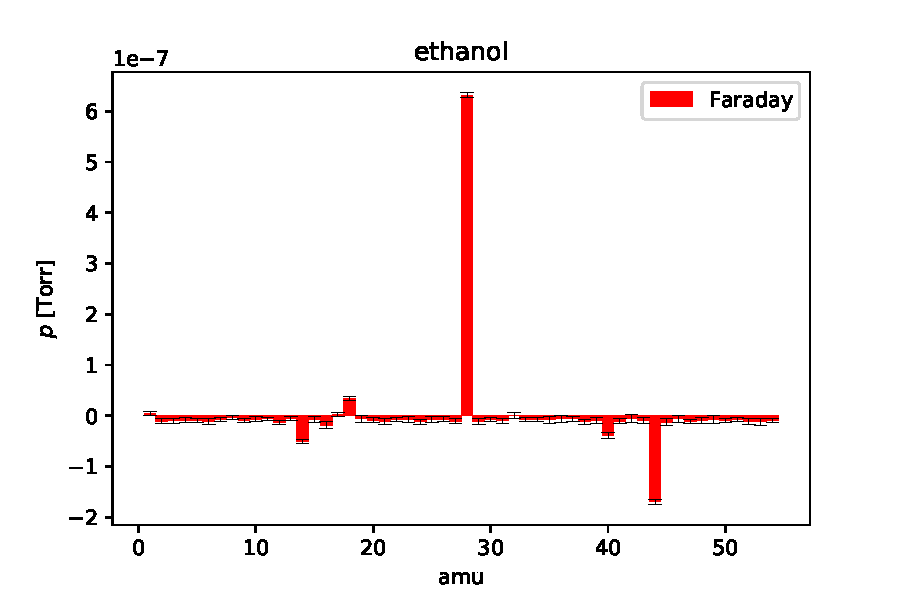
\includegraphics[width=0.65\textwidth]{Report/DataResultsPlots/ethanol.pdf}
    \caption{The measurements of our ethanol and air sample compared to first kind of \texttt{NIST} approximation.}
    \label{fig:ethanol2}
    \end{figure}
    
    %We can see that the relative peak heights are really close to the literature values gathered from the \texttt{NIST} database.
    
    \begin{figure}[h!]
    \centering
    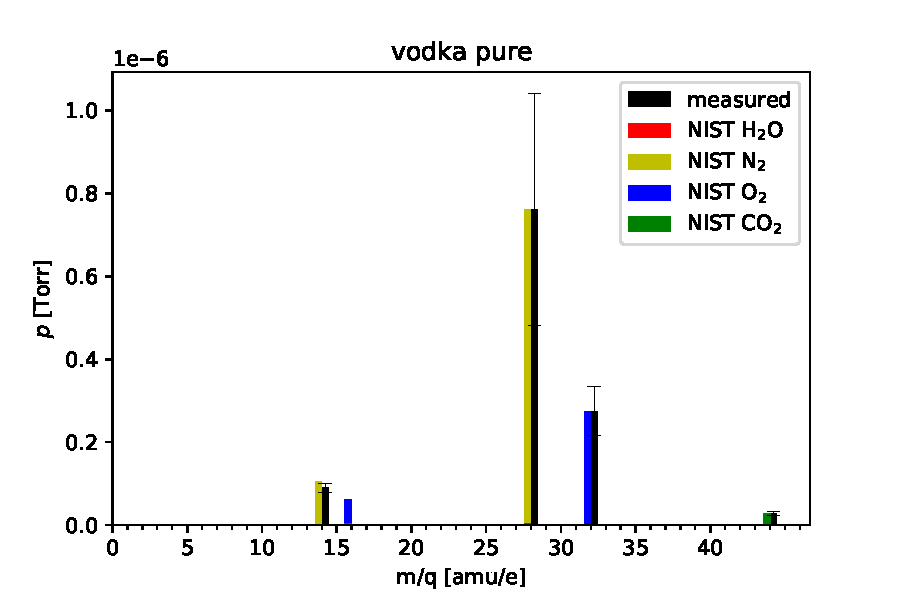
\includegraphics[width=0.65\textwidth]{Report/DataResultsPlots/vodka pure.pdf}
    \caption{The measurements of our vodka and sample compared to first kind of \texttt{NIST} approximation.}
    \label{fig:vodka}
    \end{figure}
    
    \begin{figure}[h!]
    \centering
    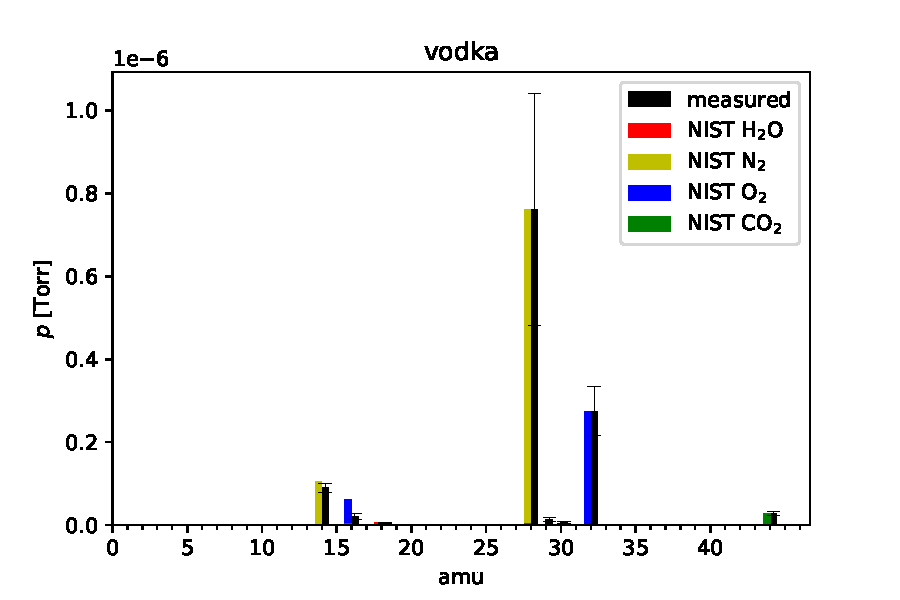
\includegraphics[width=0.65\textwidth]{Report/DataResultsPlots/vodka.pdf}
    \caption{The measurements of exhaled air after consuming vodka compared to first kind of \texttt{NIST} approximation.}
    \label{fig:vodka_air}
    \end{figure}
    
    
    As we can see, we do not detect ethanol in either type of vodka measurement (see figure \ref{fig:vodka} and \ref{fig:vodka_air}).  However, what we notice when comparing the two plots is that CO$_2$ partial pressure is higher in the exhaled air than in the direct vodka measurement and the reverse with O$_2$. This again shows that respiration consumes O$_2$ and produces CO$_2$. 
    
    
    
    \newpage
    
    \subsection{Deodorant and Sparkling Water Analysis}
    In order to measure the content of a deodorant can, we turned the can upside down and sprayed the content into a balloon. By turning it upside down we ensure that we get the propellant gas in its liquid form instead of just the fragrances and the gaseous propellant gas. The balloon was then attache to the system as shown in figure \ref{fig:setup2}.
    The measured data is compared to the \texttt{NIST} values of propane, butane isobutane and ethanol in figure \ref{fig:deo}. These components are indicated on the deodorant can. In addition, we determined the ratio of these four substances. The result can be seen in table \ref{table:deo_components}. 
    
    We also attached a balloon to a sparkling water bottle, upon shaking the bottle, the CO$_2$ started to escape and was caught in the balloon. The measurement of the balloon content is shown in figure \ref{fig:sparkling_water} and compared to the \texttt{NIST} values for CO$_2$ and other traces of elements.
    
    \begin{figure}[h]
            \centering
            \subfloat[balloon with CO2 from sparkling water]{\label{figure:sparkling}
                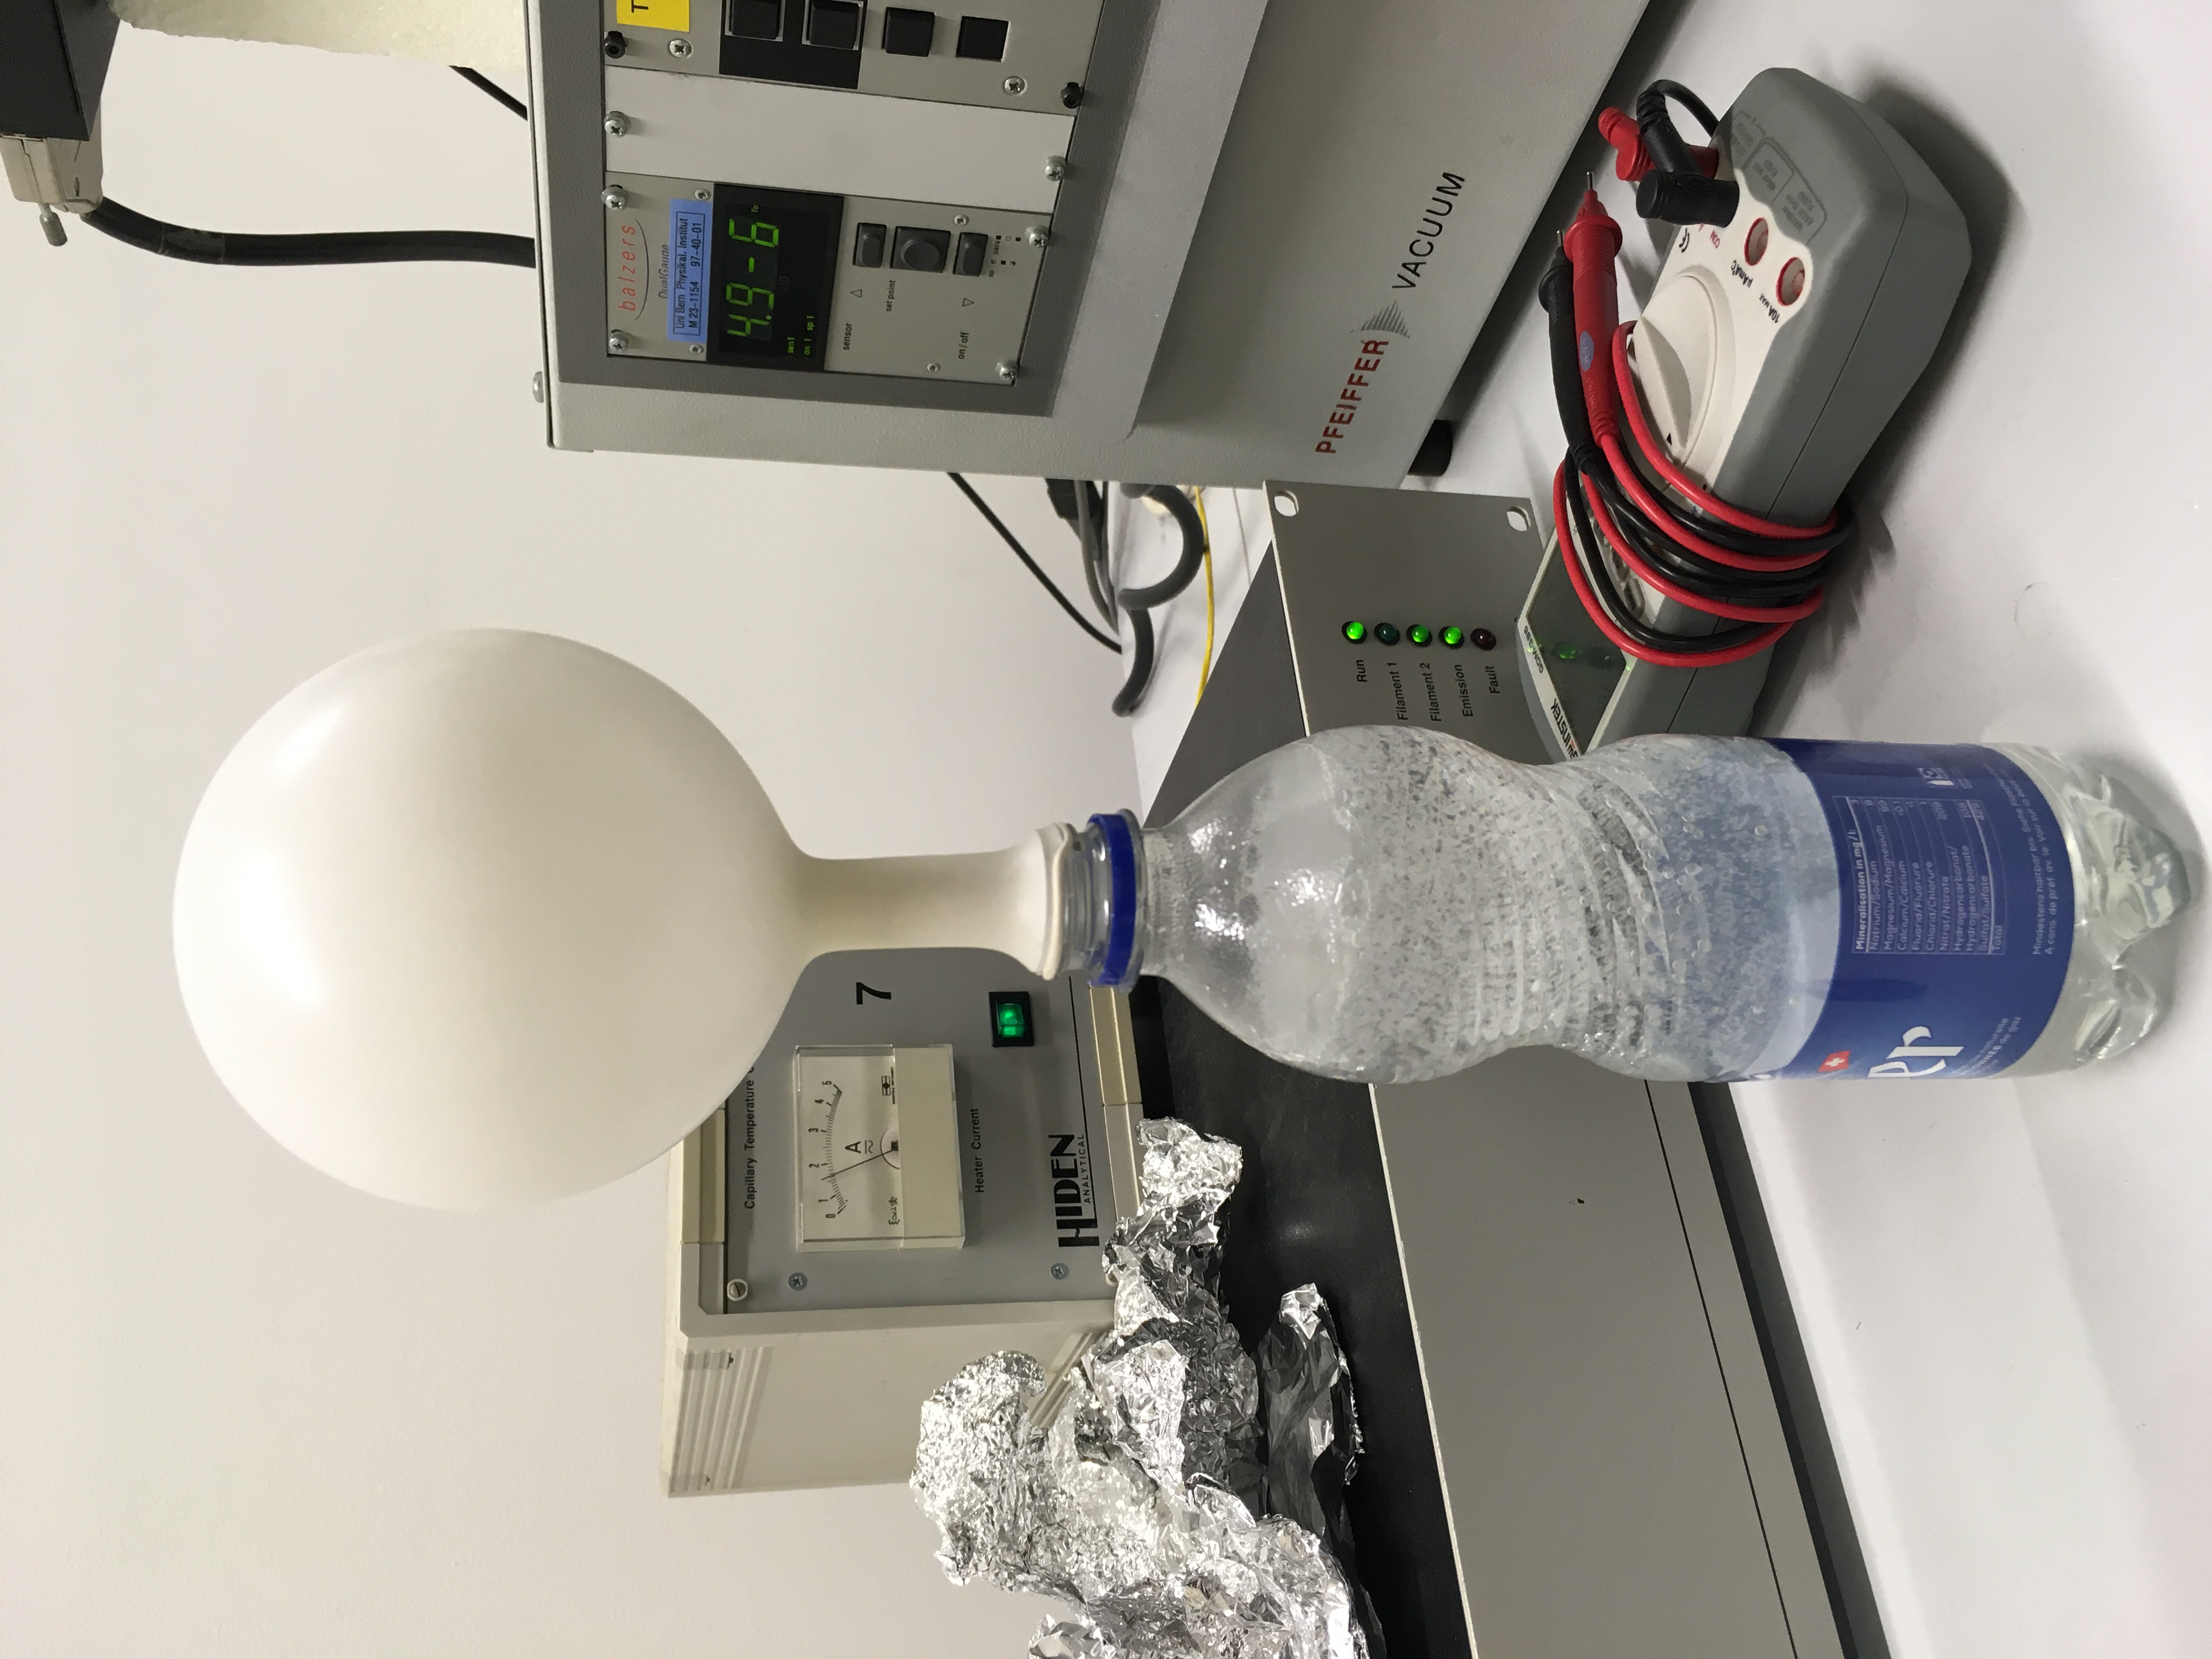
\includegraphics[width=0.47\textwidth, origin=c]{Report/pictures/ballon_bottle2.JPG}}\quad
            \subfloat[balloon attached to the system]{\label{figuer:sparkling2}
                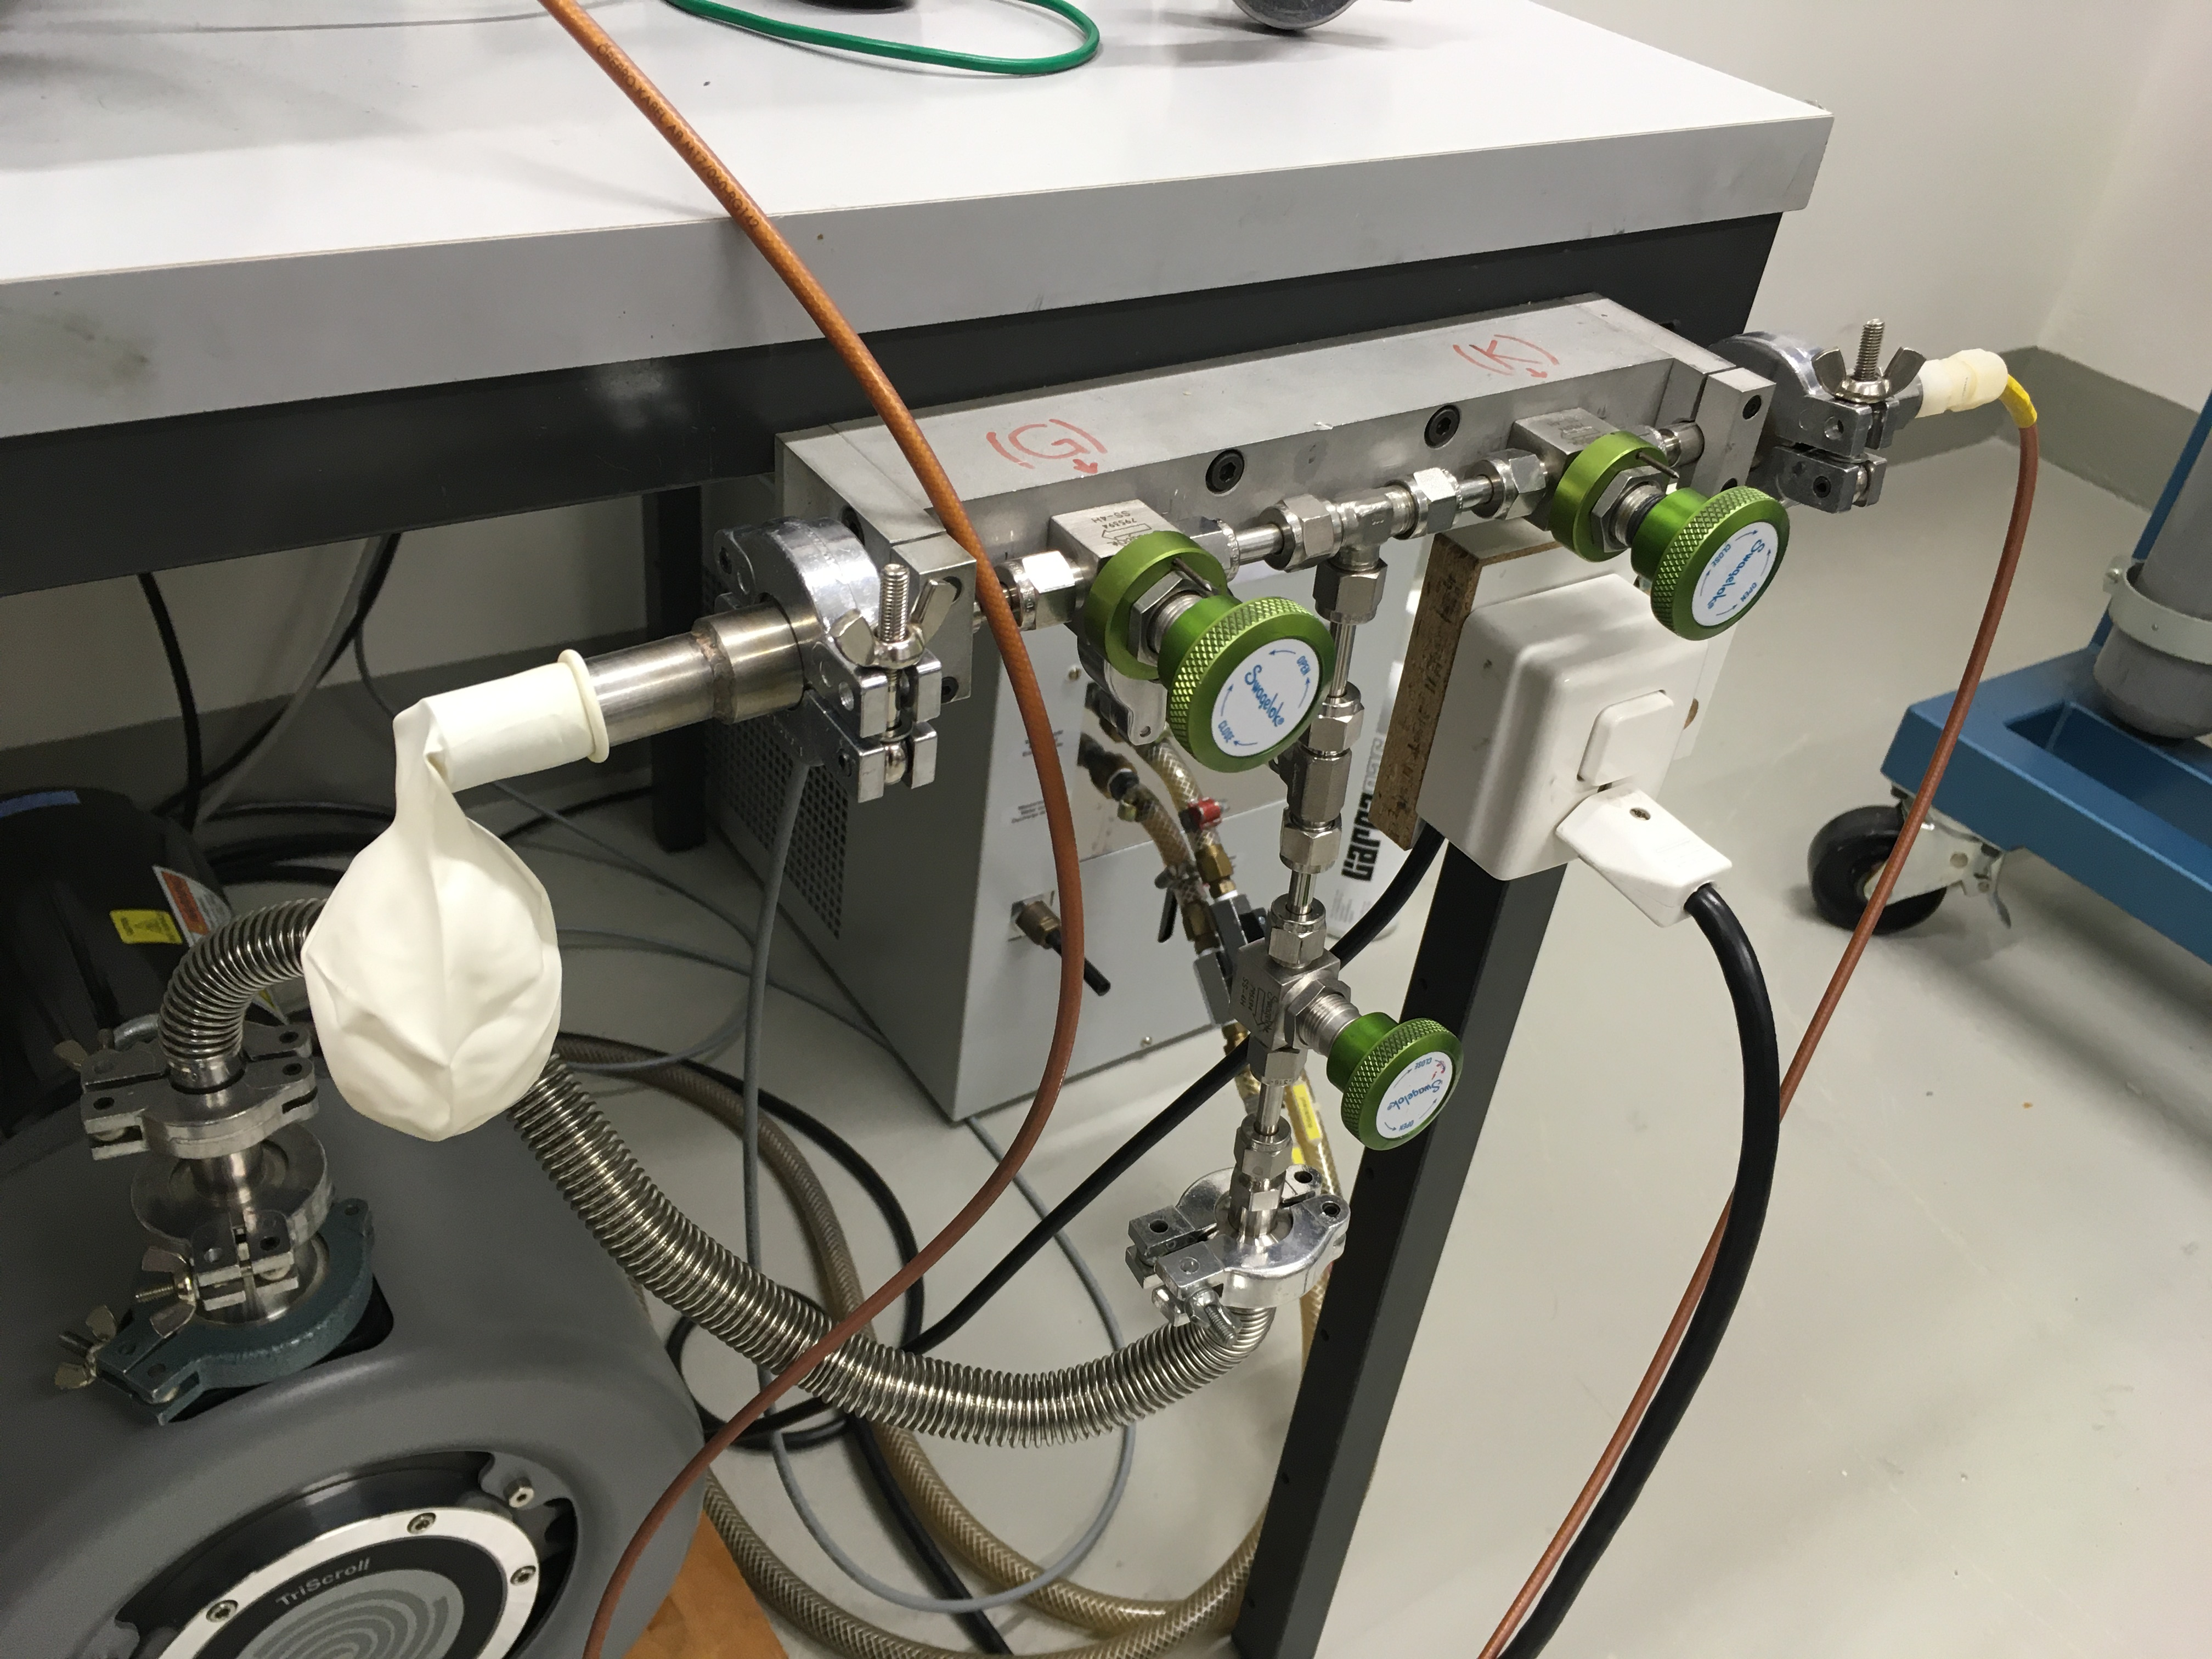
\includegraphics[width=0.47\textwidth]{Report/pictures/ballon_setup.JPG}}\quad
            \caption{The setup of the experiment with samples filled into a balloon.}
            \label{fig:setup2}
    \end{figure}

    
    \begin{figure}[h!]
    \centering
    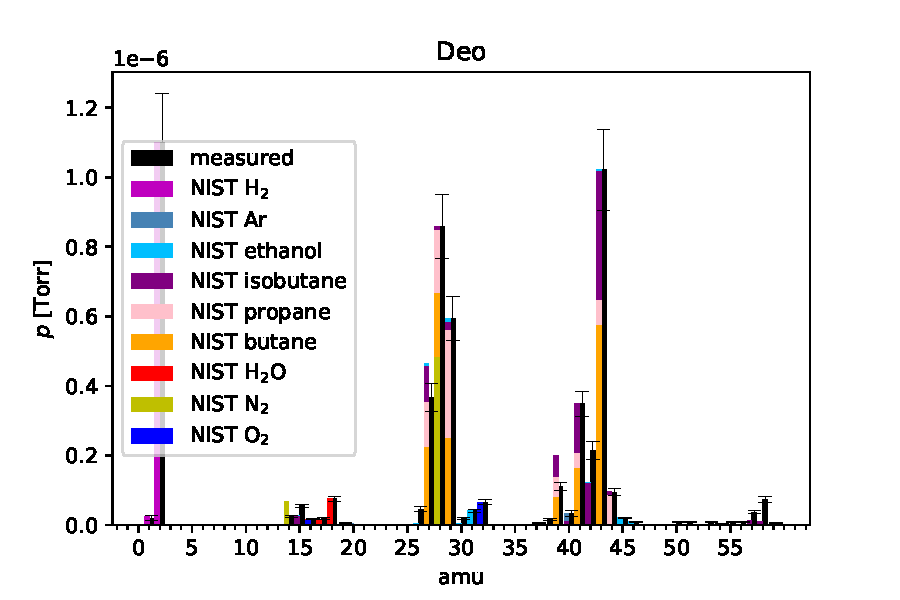
\includegraphics[width=0.7\textwidth]{Report/DataResultsPlots/deo.pdf}
    \caption{The measurements of our Deo sample compared to first kind of \texttt{NIST} approximation.}
    \label{fig:deo}
    \end{figure}
    
    
    
    \begin{table}[h!]
     \begin{center}
      \DTLsetseparator{,}
        \DTLloaddb[keys={substance,fraction,err}]{komp_deo}{komp_deo.csv}
        \begin{tabular}{l|c}
            \toprule substance & abundance [\%] 
            \DTLforeach{komp_deo}{\mat=substance,\a=fraction,\aerr=err}
            {\DTLiffirstrow{\\ \midrule}{\\}
            \mat & \pgfmathprintnumber[textnumber]\a~$\pm$~\pgfmathprintnumber[textnumber]\aerr}
            \\\bottomrule
        \end{tabular}
        \caption{Deo components}
        \label{table:deo_components}
      \end{center}
    \end{table}
    
    As we can see in table \ref{table:deo_components}, we have succeeded in detecting all four propellant gases of the deo. 
    Most of the measurements in figure \ref{fig:deo} can be well explained by the identified substances.  However, unexplained peaks between 50 amu/e and 60 amu/e are conspicuous. These could possibly be caused by fragrances. In addition, we again find a lot of H$_2$. In this case, too, it is quite conceivable that it arose from a chemical reaction from the other propellant gases.  
    
    
    
    \begin{figure}[h!]
    \centering
    \includegraphics[width=0.7\textwidth]{Report/DataResultsPlots/co_2.pdf}
    \caption{The measurements of our carbon dioxide and water sample gathered by a sparkling water bottle compared to first kind of \texttt{NIST} approximation.}
    \label{fig:sparkling_water}
    \end{figure}
    
    
    
    \begin{figure}[h!]
    \centering
    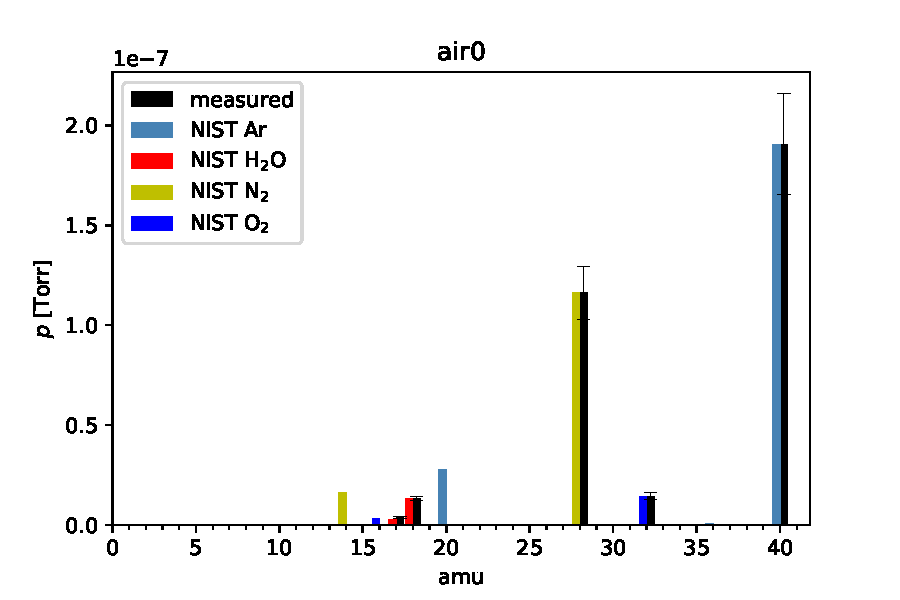
\includegraphics[width=0.7\textwidth]{Report/DataResultsPlots/air0.pdf}
    \caption{The measurements of indoor air compared to first kind of \texttt{NIST} approximation.}
    \label{fig:air0}
    \end{figure}
    
    As we can see in figure \ref{fig:sparkling_water}, a very large proportion of CO$_2$ in the sparkling water measurement was indeed detected. In order to be able to compare this CO$_2$ content, a measurement of pure air is shown in figure \ref{fig:air0}. We find that they only differ in the CO$_2$ occurrence in the sparkling water plot. Although there is a clear argon peak in the room air, this is due to residual gases from the noble gas measurements conducted before. 
    \FloatBarrier
    